
Proces przetwarzania możemy opisać i analizować jako współpracę obiektów dwu klas: neuronu (\textit{Neuron}) i warstwy (\textit{Layer}). Ujęcie obiektowe umożliwia ściślejszą hermetyzację, ułatwia realizację współbieżności przetwarzania. Realizacja w tym modelu umożliwia wykorzystanie wzorców projektowych w tym: \textit{dziedziczenia}, \textit{interfejsu} czy \textit{obserwatora}.

\section{ Obiekt klasy Layer }

\begin{figure}[h]
	\centering 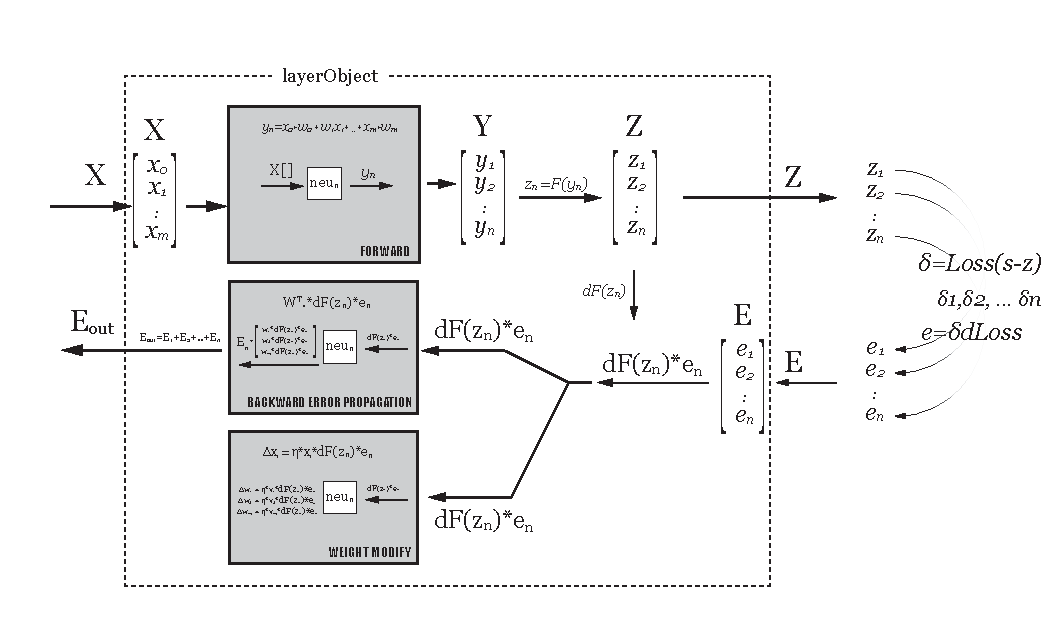
\includegraphics[width=\textwidth]{gfx/rys1_4.pdf} 
	\caption{ Przepływu sygnałów w obiekcie Layer  }
	\label{rys:modelobiektowegoneuronuszkic1}
\end{figure}

Każdy obiekt Layer ma własną kolekcję obiektów klasy Neuron. Dysponuje też polami danych np. X, które są zbiorami wartości. I tak pole danych X jest zbiorem wartości { \(x_0, x_1, ... x_m \) }. pole danych Y jest zbiorem wartości { \(y_0, y_1, ... y_m \) }. Z matematycznego punktu widzenia, można powiedzieć że wektor X jest wektorem zmiennych niezależnych X = [ \(x_0, x_1, ... x_m \) ], skoro tak, to i \textbf{pochodne składników tych wektorów będą niezależne względem siebie}. Z informatycznego punktu widzenia pole X jest zbiorem wartości  \(x_0, x_1, ... x_m \), które może być realizowane przez takie struktury danych jak \textit{zbiór}, \textit{lista}, \textit{tablica} czy \textit{wektor}. Zależnie od języka programowania pewne struktury będą wygodniejsze do wykorzystania od innych. Struktura \textit{tablica} jest najprostsza, kolejne wartości są indeksowane liczbą całkowitą, a sama tablica po utworzeniu nie może zmieniać swojego rozmiaru. 

Obiekty klasy Layer wywołuje dla wszystkich neuronów ze swojej kolekcji żądania wykonania obliczeń. Obiekty klasy Neuron mają dostęp do obiektu rodzica, a dzięki temu mają także dostęp do niektórych pól danych obiektu Layer. Neurony nie mają jednak bezpośrednich połączeń między sobą. 







\begin{figure}[h]
	\centering 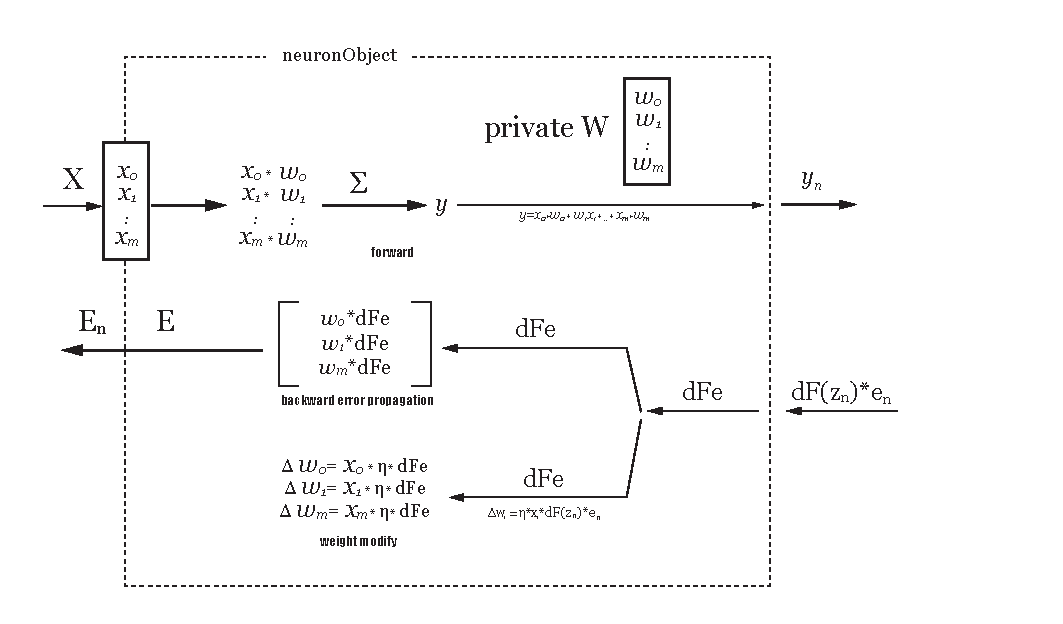
\includegraphics[width=\textwidth]{gfx/rys1_5.pdf} 
	\caption{ Przepływu sygnałów w obiekcie Neuron }
	\label{rys:modelobiektowegoneuronuszkic2}
\end{figure}

Obiekty klasy Neuron są bardzo proste i lekkie, realizują kilka operacji matematycznych wywoływanych na żądanie warstwy rodzica. Do obliczeń używają wewnętrznych zmiennych wag zorganizowanych w tablicę \( W = [ w_0, w_1, ... w_m ]\) , oraz dostarczonych przez rodzica zmiennych skalarnych oznaczanych małymi lierami np. \(\eta\), lub tablic skalarów oznaczanych dla rozróżnienia wielkimi literami np. pole X. 
 
\newpage
\begin{figure}[h]
	\centering 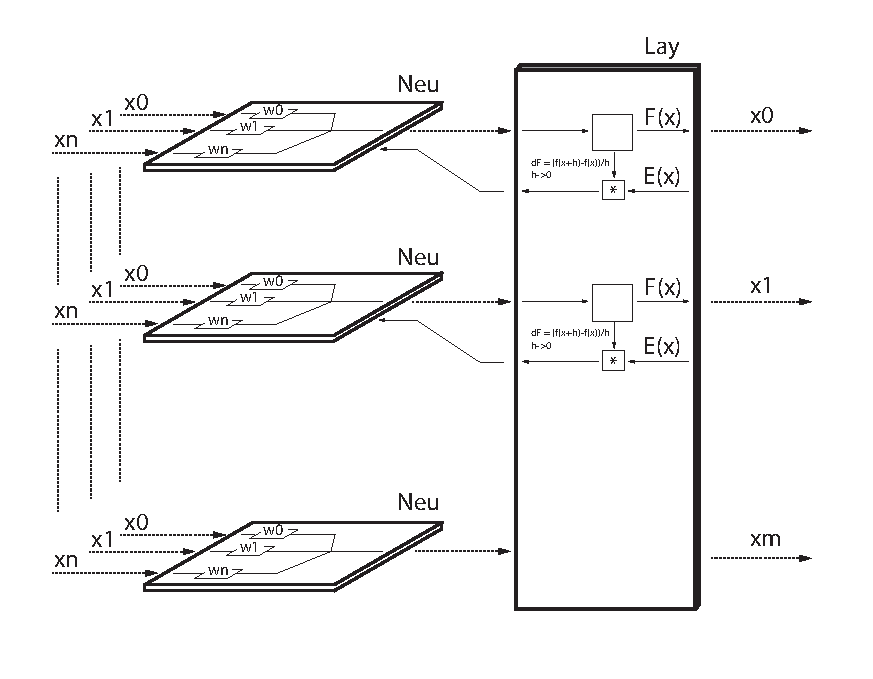
\includegraphics[width=0.5\textwidth]{gfx/3d.pdf} 
	\caption{ współpraca klas Neuron / Layer }
	\label{rys:modelobiektowegoneuronuszkic2}
\end{figure}
\section{ Propagacja sygnału pomiędzy obiektami }
Pojedynczy neuron odczytuje wartości wektora wejściowego - tablicy \(X\) o określonym rozmiarze \(m\), przekazanego przez rodzica. Oblicza iloczyn odpowiednich wag i wartości, a następnie sumuje uzyskane iloczyny. Obliczoną \textbf{wartość skalarną zmiennoprzecinkową} - zwraca jako wynik operacji.
\newline
\begin{lstlisting}
    public float forward( float[] X ) {
        float sum=0;
        for ( int m=0; m<W.length; m++ ) {
            yi= X[m]*W[m];
            sum = sum + yi;
        }
        return sum;
    }
\end{lstlisting}
obiekt Layer dla otrzymanych wartości \(y_1, y_2, ... y_n\) oblicza wielkość funkcji aktywacji \(z_i = f(y_i)\). 
Metoda wyliczająca wielkość funkcji aktywacji zależnie do rodzaju warstwy:
\begin{lstlisting}
    private float F ( float y ){
        float z;
        switch (this.lType) {
            case sigmod: { return ( 1/(1 + Math.exp( -y ))); }
            case linear:
                default: { z=y; break; }
        }
        return z;
    }
\end{lstlisting}

Wielkości te zebrane w tablicę tworzą wartość wyjściową Z. 
Przy okazji obliczamy także wartość pochodnych funkcji F w punktach \(y_i\) i zapisujemy w tablicy dFofZ).

\begin{lstlisting}
    public void forward(){
        for ( int n=0; n<neurons.length; n++ ) {
            Y[n] = neurons[n].forward( X );
            Z[n] = F ( Y[n] );
            dFofZ[n] = dF( Z[n] );
        }
    }
\end{lstlisting}

Zestawienie pochodnych funkcji straty \(Loss\) oraz funkcji aktywacji \(dF(y)\) zależnie od rodzajów warstw ~\ref{tab:funkcjeaktywacji}.

\begin{lstlisting}
    private float dF (float z ){
        float df;
        switch (lType) {
            case sigmod: { df = z*(1-z); break; }
            case linear:
            default: { df=1; break; }
        }
        return df;
    }
\end{lstlisting}


Pierwsze programy napisane przy użyciu modelu wykonują poprawnie przykładowe zadania z \cite{profWłodzimierzKasprzak2024wyklad}.





